\documentclass[First Project.tex]{subfiles}
\begin{document}

\subsection{ Τροποποιημένη μέθοδος \textlatin{Newton-Raphson} }

Στην τροποποιημένη μέθοδο \textlatin{Newton-Raphson} αλλάζει ο αναδρομικός τύπος της ακολουθίας για την εκτίμηση της ρίζας. Η συνάρτηση 
\textit{\textlatin{\textbf{modified\_newton\_raphson}}} από το αρχείο \textit{\textlatin{\textbf{modified\_newton\_raphson.py}}} δέχεται τα 
ίδια ορίσματα με την κλασσική μέθοδο \textlatin{Newton-Raphson}.
\begin{figure}[h!]
    \centering
    \captionsetup{justification=centering}
    \begin{center}
        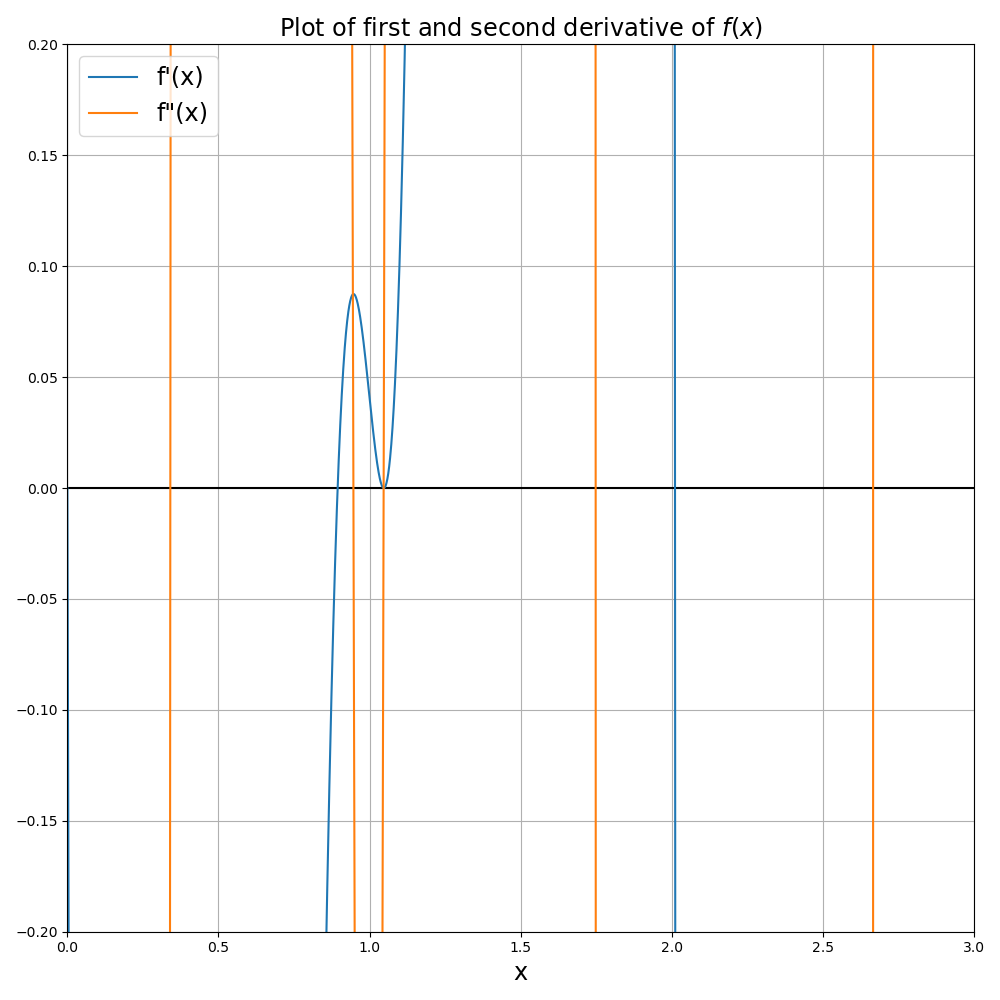
\includegraphics[scale=0.40]{exercise_2_function_derivatives.png}    
        \caption{Γραφική παράσταση της πρώτης και δεύτερης παραγώγου της συνάρτησης \textlatin{\textbf{f(x)}}}
    \end{center}
\end{figure}

Για την πρώτη ρίζα της \textlatin{\textbf{f(x)}} στο διάστημα επιλέγουμε \textlatin{\textbf{ $x_{0}$ = 0.5}} όπου τηρούνται όλες οι προϋποθέσεις
για την μέθοδο \textlatin{\textbf{Newton-Raphson}}. 
\begin{figure}[h!]
    \centering
    \captionsetup{justification=centering}
    \begin{center}
        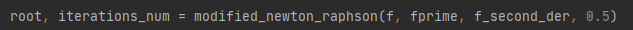
\includegraphics[scale=0.7]{exercise_2_newton_call_first_root.png}    
        \caption{Παράδειγμα κλήσης της συνάρτησης \textit{\textlatin{\textbf{modified\_newton\_raphson}}}.}
    \end{center}
\end{figure}
Μετά την κλήση της συνάρτησης έχουμε τα παρακάτω αποτελέσματα :
\begin{figure}[h!]
    \centering
    \captionsetup{justification=centering}
    \begin{center}
    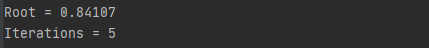
\includegraphics[scale=1]{exercise_2_newton_result_first_root.png}    
    \caption{ Αποτελέσματα κλήσης της συνάρτησης \textit{\textlatin{\textbf{modified\_newton\_raphson}}} \\ με αρχικό σημείο 
                \textlatin{\textbf{$x_{0}$ = 0.5}}}.
    \end{center}
\end{figure}

Όπου παρατηρούμε ότι η ρίζα της \textlatin{\textbf{f(x)}} στο διάστημα \textbf{[0.5,1.0]} με ακρίβεια 5 δεκαδικών ψηφίων 
είναι η \textbf{0.84107} (εμφάνιση με στρογγυλοποίηση στο 5ο δεκαδικό) καθώς και ότι η τροποποιημένη μέθοδος \textlatin{\textbf{Newton-Raphson}} χρειάστηκε \textbf{5} επαναλήψεις για να επιτύχει την 
επιθυμητή ακρίβεια. Για την ρίζα της συνάρτησης στο διάστημα \textbf{[2.0,2.5]} επιλέγουμε \textlatin{\textbf{ $x_{0}$ = 2.5}} όπου τηρούνται 
όλες οι προϋποθέσεις για την μέθοδο \textlatin{\textbf{Newton-Raphson}}. 
\begin{figure}[h!]
    \centering
    \captionsetup{justification=centering}
    \begin{center}
        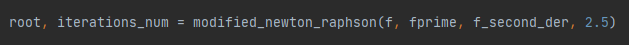
\includegraphics[scale=0.7]{exercise_2_newton_call_third_root.png}    
        \caption{Παράδειγμα κλήσης της συνάρτησης \textit{\textlatin{\textbf{modified\_newton\_raphson}}}.}
    \end{center}
\end{figure}

Μετά την κλήση της συνάρτησης έχουμε τα παρακάτω αποτελέσματα :

\begin{figure}[h!]
    \centering
    \captionsetup{justification=centering}
    \begin{center}
    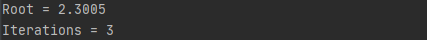
\includegraphics[scale=1]{exercise_2_newton_result_third_root.png}    
    \caption{ Αποτελέσματα κλήσης της συνάρτησης \textit{\textlatin{\textbf{modified\_newton\_raphson}}} \\ με αρχικό σημείο 
                \textlatin{\textbf{$x_{0}$ = 0.5}}}.
    \end{center}
\end{figure}

Όπου παρατηρούμε ότι η ρίζα της \textlatin{\textbf{f(x)}} στο διάστημα \textbf{[2.0,2.5]} με ακρίβεια 5 δεκαδικών ψηφίων 
είναι η \textbf{2.3005} καθώς και ότι η τροποποιημένη μέθοδος \textlatin{\textbf{Newton-Raphson}} χρειάστηκε \textbf{3} επαναλήψεις για να επιτύχει την 
επιθυμητή ακρίβεια. Τέλος, για την ρίζα της \textlatin{\textbf{f(x)}} στο διάστημα \textbf{[1.0,1.25]} αν υπολογίσουμε τις τιμές της πρώτης
και δεύτερης παραγώγου θα δούμε ότι μηδενίζονται και αυτές. Επομένως, η ρίζα αυτή έχει πολλαπλότητα \textlatin{\textbf{m = 3}} και δεν
τηρούνται όλες οι προϋποθέσεις για την μέθοδο \textlatin{\textbf{Newton-Raphson}} και είτε δεν θα έχουμε καθόλου σύγκλιση είτε 
σύγκλιση αλλά όχι με την επιθυμητή ακρίβεια. Για παράδειγμα, αν δοκίμασουμε να καλέσουμε την συνάρτηση με αρχικό σημείο το 
\textlatin{\textbf{ $x_{0}$ = 1.04}} ( ένα σημείο αρκετά κοντά στην ρίζα ) 
\begin{figure}[h!]
    \centering
    \captionsetup{justification=centering}
    \begin{center}
    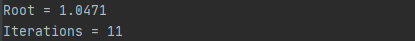
\includegraphics[scale=1]{exercise_2_newton_result_second_root.png}    
    \caption{ Αποτελέσματα κλήσης της συνάρτησης \textit{\textlatin{\textbf{modified\_newton\_raphson}}} \\ με αρχικό σημείο 
                \textlatin{\textbf{$x_{0}$ = 1.04}}}.
    \end{center}
\end{figure}
παρατηρούμε στο \textit{Σχήμα 33} ότι δεν έχουμε την επιθυμητή ακρίβεια ( εμφάνιση με στρογγυλοποίηση στο 5ο δεκαδικό).
\end{document}